%%%%%%%%%%%%%%%%%%%%%%%%%%%%%%%%%%%%%%%%%
% IST Poster
% LaTeX Template
% Version 1.0 (17/08/2017)
% (Based on Version 1.0 (31/08/2015) of the Jacobs Portrait Poster
%
% License:
% CC BY-NC-SA 3.0 (http://creativecommons.org/licenses/by-nc-sa/3.0/)
%
% Created by:
% Francisco Maria Calisto, IST, Universidade de Lisboa
% francisco.calisto@tecnico.ulisboa.pt
% http://tecnico.ulisboa.pt/
%%%%%%%%%%%%%%%%%%%%%%%%%%%%%%%%%%%%%%%%%


\def\footer#1{\def\insertfooter{#1}}
%--------------------------------------------------------------------------------------
%	PACKAGES AND OTHER DOCUMENT CONFIGURATIONS
%--------------------------------------------------------------------------------------

\documentclass[final]{beamer}
% Load basic packages
\usepackage{balance}  % to better equalize the last page
\usepackage{amssymb}  % mathematical symbols
\usepackage{graphics} % for EPS, load graphicx instead
\usepackage{pgfplots} % Bar charts
\usepackage{times}    % comment if you want LaTeX's default font
\usepackage{url}      % llt: nicely formatted URLs
\usepackage[utf8]{inputenc}
\usepackage{soul}
\sethlcolor{black}

\usepackage{tikz}
\usepackage{subcaption}

\usepackage[scale=1.150]{beamerposter} % Use the beamerposter package
\usetheme{MUWposter} % Use the MUWposter theme supplied with this template

% Include a logo of your project if desired
\logo{\pgfputat{\pgfxy(-11,107)}{\pgfbox[center,base]{
\includegraphics[width=7cm]{logo.png}}}}

\usepackage{multicol}
\usepackage{array}
%The following two are column definitions for the aknowledgements section
\newcolumntype{L}{>{\arraybackslash}m{22cm}}
\newcolumntype{S}{>{\arraybackslash}m{5cm}}
\usepackage{pgf}  
\usepackage{mathtools}
\usepackage{amsmath, amsthm, amssymb, amsfonts}
\usepackage{exscale}
\usepackage{xcolor}
\usepackage{ushort}
\usepackage{setspace}
\usepackage[square,numbers]{natbib}
\usepackage{url}
\bibliographystyle{abbrvnat}
\renewcommand{\vec}[1]{\ushort{#1}}
\renewcommand{\vec}[1]{\mathbf{#1}}
\definecolor{greenMUW}{RGB}{60,191,174}
\definecolor{blueMUW}{RGB}{17,29,79}
\definecolor{skinMUW}{RGB}{254,228,217}
\definecolor{hellblauMUW}{RGB}{95,180,229}

%-----------------------------------------------
%  START Set the colors
%  Uncomment to apply colors you want to use.
%-----------------------------------------------
\colorlet{themecolor}{greenMUW}
\usebackgroundtemplate{
\includegraphics{green.pdf}}

%\colorlet{themecolor}{skinMUW}
%\colorlet{themecolor}{blueMUW}
%\usebackgroundtemplate{
\includegraphics{MUW_skin.pdf}}

%%\colorlet{themecolor}{blueMUW}
%\colorlet{themecolor}{hellblauMUW}
%\usebackgroundtemplate{
\includegraphics{MUW_hellblau.pdf}}
%-----------------------------------------------
%  END Set the colors
%-----------------------------------------------


%-----------------------------------------------
%  START Set the width of the columns
%-----------------------------------------------
\setlength{\paperwidth}{33.1in} % A0 width: 46.8in
\setlength{\paperheight}{46.8in} % A0 height: 33.1in
\newlength{\sepmargin}
\newlength{\sepwid}
\newlength{\onecolwid}
\newlength{\twocolwid}
\newlength{\threecolwid}

% The following measures are used for 2 columns
\setlength{\sepmargin}{0.055\paperwidth} % Separation width (white space) between columns
\setlength{\sepwid}{0.03\paperwidth} % Separation width (white space) between columns
\setlength{\onecolwid}{0.43\paperwidth} % Width of one column
\setlength{\twocolwid}{0.9\paperwidth} % Width of two columns

%-----------------------------------------------------------
% The following measures are used for 3 columns
%\setlength{\sepmargin}{0.06\paperwidth} % Separation width (white space) between columns
%\setlength{\sepwid}{0.02\paperwidth} % Separation width (white space) between columns
%\setlength{\onecolwid}{0.28\paperwidth} % Width of one column
%\setlength{\twocolwid}{0.58\paperwidth} % Width of two columns
%\setlength{\threecolwid}{0.88\paperwidth} % Width of three columns
%\setlength{\columnsep}{30pt}

%-----------------------------------------------
%  END Set the width of the columns
%-----------------------------------------------


%--------------------------------------------------------------------------------------
%	TITLE SECTION 
%--------------------------------------------------------------------------------------
\setbeamertemplate{title}[left]
\setbeamertemplate{frametitle}[default][left]
%\setmainfont{Georgia}

\title{Towards Touch-Based Medical Image Diagnosis Annotation} % Poster title

\author{Francisco Maria Calisto, Jacinto Carlos Nascimento, Alfredo Ferreira, Daniel Gon\c{c}alves} % Author(s)

\institute{Institute for Systems and Robotics (ISR/IST), LARSyS, INESC-ID, Instituto Superior T\'{e}cnico, Universidade de Lisboa} % Institution(s)
%------------------------------------------------------------------



\begin{document}

\addtobeamertemplate{block end}{}{\vspace*{1ex}} % White space under blocks
\addtobeamertemplate{block alerted end}{}{\vspace*{0ex}} % White space under highlighted (alert) blocks
\setlength{\belowcaptionskip}{2ex} % White space under figures
\setlength\belowdisplayshortskip{1ex} % White space under equations


\begin{frame}[t] % The whole poster is enclosed in one beamer frame

\begin{columns}[t] % The whole poster consists of two major columns

\begin{column}{\sepmargin}\end{column}

\begin{column}{\onecolwid} % The first column


\begin{block}{Abstract}
%\begin{multicols}{2}

A fundamental step in medical diagnosis for patient follow-up relies on the ability of radiologists performing reliable diagnosis from acquired images. Basically, the diagnosis strongly depends on the visual inspection over the shape of the lesions, and somehow register its evolution through time. As datasets increase in size, such visual evaluation becomes harder. For this reason it is crucial to introduce easy-to-use interfaces that help the radiologists not only to perform a reliable visual inspection but more importantly, allow the efficient delineation of the lesions. In this paper, we will present a study on integrating the above interfaces in a real-world scenario. More specifically, we will explore the radiologist's receptivity to the current touch environment solution. The advantages of touch are threefold: (i) the time performance is superior regarding the traditional use, (ii) it has more intuitive control and, (iii) for less time, the user interface delivers more information per action, concerning annotations. We concluded, from our studies that the path towards touch-based on medical image diagnosis annotation includes overcoming the current refusal to use these systems by radiologists, which resist change. Also, a solution to the finger occlusion must be devised.

%\end{multicols}
\end{block}

\begin{block}{Evaluation}
%\begin{multicols}{2}

We measure accuracy by computing the Hit Rate Score (HRS). This measure is defined has the percentage of annotations that lie on three areas. These three areas are measured from the ground-truth. The first area, \textbf{Area A}, is the area delimited by the two \textbf{Green Lines}, having a width of $2\epsilon$, where $\epsilon$ is the perpendicular distance from a point in the ground truth (black line) to the \textbf{Green Line}. The second area, \textbf{Area B}, has also a width of $2\epsilon$. However,  \textbf{Area B} embraces two regions, each region falling between the \textbf{Green Lines} (inner boundary) and \textbf{Red Lines} (outer boundary).

\begin{figure}
  \begin{center}
  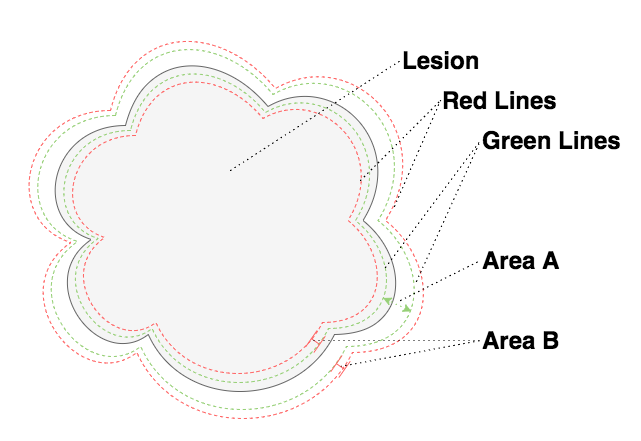
\includegraphics[width=25cm]{mimbcd-ui_areas.png}
  \end{center}
\end{figure}

%\end{multicols}
\end{block}

\begin{block}{Conclusion}
%\begin{multicols}{2}

In this work, we propose and evaluate a set of results to a medical image diagnosis user interface on traditional and touch environments. Our analysis describes performance and experience on both environments using a simple user interface and several validated scales. We fully describe our proposed interaction design techniques and detail the aspects of our user interface interaction.

%\end{multicols}
\end{block}

\end{column}



\begin{column}{\sepwid}  \end{column}




\begin{column}{\onecolwid} %The second column

\begin{block}{ }

Our research is applied to a novel domain: the medical image diagnosis; where touch user interface produces a superior time performance regarding  the traditional use. Also, it has more intuitive control and a higher number of interactions, giving a more information concerning the annotation of the lesions in shorter time.

\begin{figure}
\begin{tikzpicture}
    \begin{axis}[
        ybar,
        every node near coord/.append style={rotate=90, anchor=west},
        ymin=0,
        width  = 35cm,
        height = 20cm,
        bar width=50pt,
        nodes near coords,
        xticklabel style={rotate=0},
        xtick = data,
        table/header=false,
        table/row sep=\\,
        xticklabels from table={
          1\\2\\3\\4\\5\\
          }{[index]0},
        enlarge y limits={value=1.00,upper},
        legend pos=north west
    ]
    \addplot table[x expr=\coordindex,y index=0]{35.46\\29.50\\37.27\\37.73\\25.04\\};
    \addplot table[x expr=\coordindex,y index=0]{37.77\\32.42\\33.65\\32.88\\28.27\\};
    \legend{Traditional, Touch}
    \end{axis}
\end{tikzpicture}
\caption{Kruskal-Wallis.}
\label{fig:Fig8}
\end{figure}

\begin{figure}
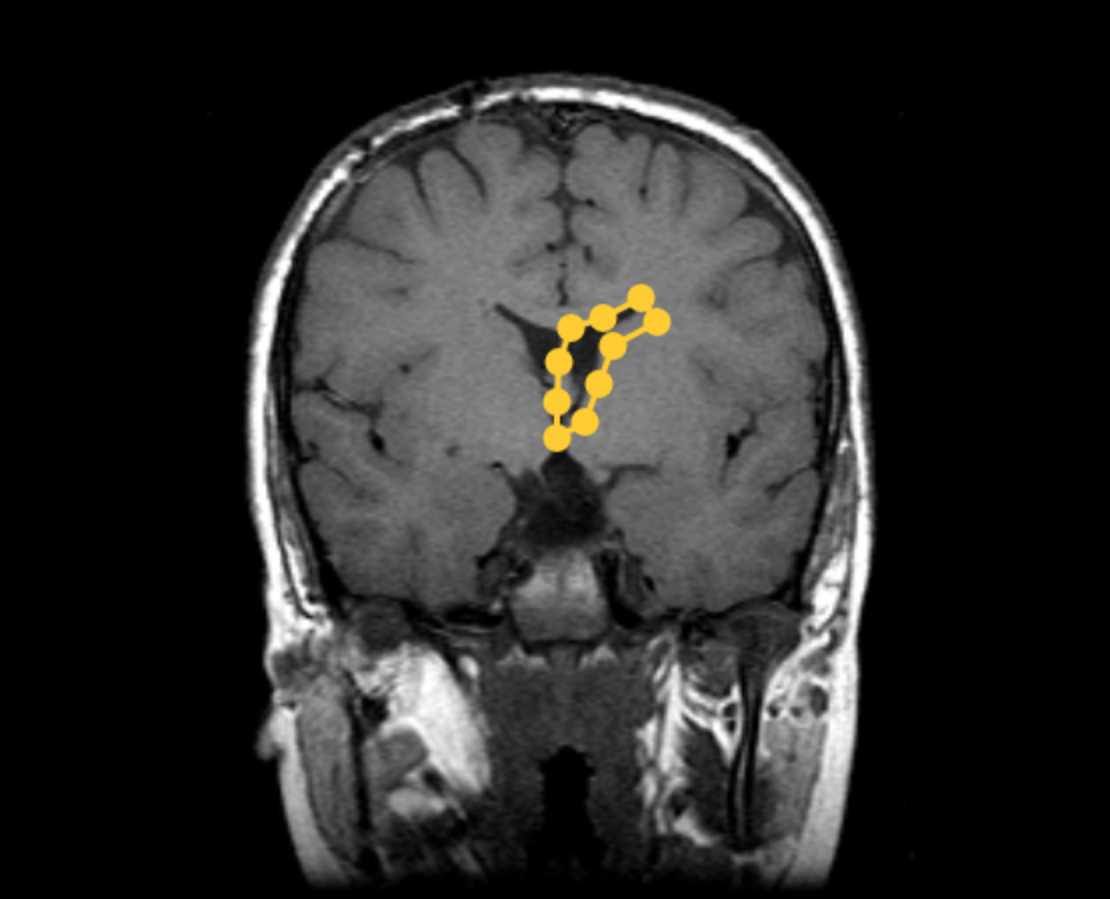
\includegraphics[width=.9\linewidth]{screen4.png}
\end{figure}

\begin{multicols}{2}
\begin{figure}
\vspace*{-0.95cm}
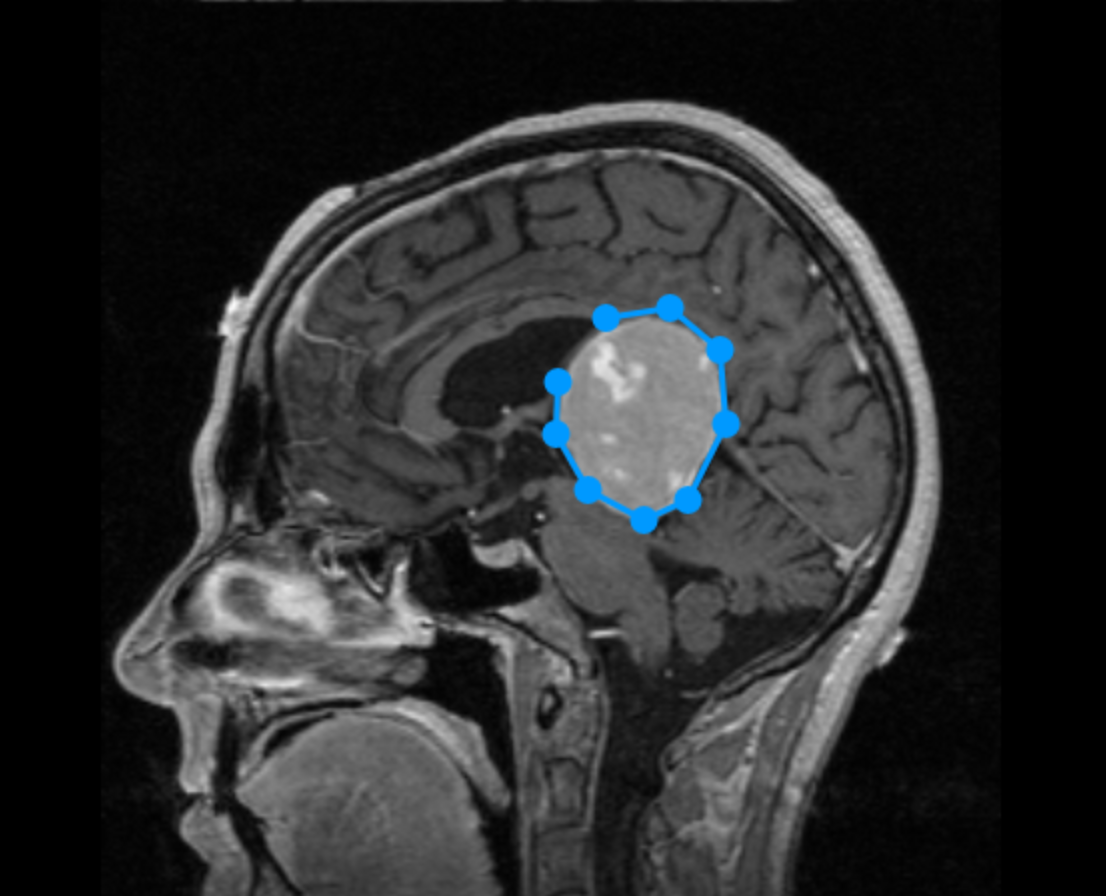
\includegraphics[width=.8\linewidth]{screen2.png}
\end{figure}
\begin{figure}
\vspace*{-0.95cm}
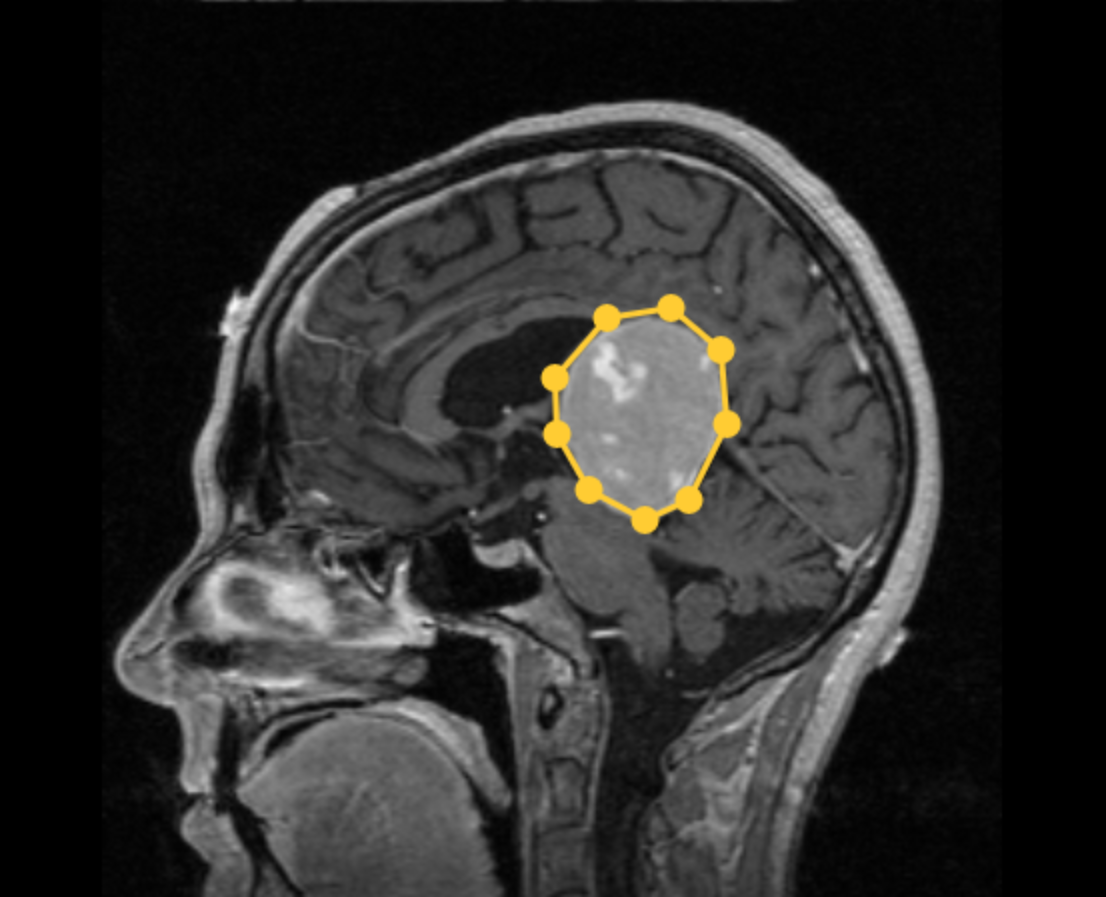
\includegraphics[width=.8\linewidth]{screen3.png}
\end{figure}
\end{multicols}

\end{block}
\end{column}

\begin{column}{\sepmargin} \end{column}
\end{columns} 

\begin{columns}[t] % Split up the two columns wide column again

\begin{column}{\sepmargin} \end{column}
\begin{column}{\onecolwid} % The first column
\begin{block}{\large Sponsors}
\begin{tabular}{SL}

\includegraphics[height=2.5cm]{Flag_of_Europe.png}
\hspace*{0.50cm}

\includegraphics[height=2.5cm]{republica_portuguesa.png}
\hspace*{0.50cm}

\includegraphics[height=2.5cm]{fct.png}
\hspace*{0.50cm}

\includegraphics[height=2.5cm]{fccn.png}
&
\end{tabular}
\begin{tabular}{SL}

\includegraphics[height=2.5cm]{ulisboa.png}
\hspace*{0.50cm}

\includegraphics[height=2.5cm]{IST_C_RGB_POS.png}
\hspace*{0.50cm}

\includegraphics[height=2.5cm]{DEI_RGB.png}
\hspace*{0.50cm}

\includegraphics[height=2.5cm]{logo-inesc-id.png}
\hspace*{0.50cm}

\includegraphics[height=2.5cm]{logo_200.png}
&
\end{tabular}

\begin{alertblock}{\small Contact Information}
\vspace*{-0.75cm}
\begin{footnotesize}
\begin{itemize}
\item \href{mailto:francisco.calisto@tecnico.ulisboa.pt}{francisco.calisto@tecnico.ulisboa.pt}
\item \href{https://mimbcd-ui.github.io/}{mimbcd-ui.github.io} - \href{https://tecnico.ulisboa.pt/}{tecnico.ulisboa.pt}
\end{itemize}
\end{footnotesize}
\end{alertblock}

\end{block}	
\vspace*{-1.25cm}

\end{column} % End of the first column
\begin{column}{\sepwid}\end{column} % Empty spacer column
\begin{column}{\onecolwid} % Begin a column

\begin{block}{\large References}
\vspace*{-0.5cm}
\nocite{*} % Insert publications even if they are not cited in the poster
{\footnotesize
%\bibliographystyle{plainurl}
\bibliography{bibliog.bib}}
\end{block} 
\end{column} % End of the second column

\begin{column}{\sepmargin}\end{column} % Empty spacer column

\end{columns} % End of all the columns in the poster


\end{frame} % End of the enclosing frame

\end{document}
